\documentclass[a4paper,10pt]{article}
\usepackage[brazilian]{babel}
\usepackage[left=2.5cm,right=2.5cm,top=3cm,bottom=2.5cm]{geometry}
\usepackage{mathtools}
\usepackage{amsthm}
\usepackage{amsmath}
%\usepackage{nccmath}
\usepackage{amssymb}
\usepackage{amsfonts}
\usepackage{physics}
%\usepackage{dsfont}
%\usepackage{mathrsfs}

\usepackage{titling}
\usepackage{indentfirst}

\usepackage{bm}
\usepackage[dvipsnames]{xcolor}
\usepackage{cancel}

\usepackage{xurl}
\usepackage[colorlinks=true]{hyperref}

\usepackage{float}
\usepackage{graphicx}
%\usepackage{tikz}
\usepackage{caption}
\usepackage{subcaption}

%%%%%%%%%%%%%%%%%%%%%%%%%%%%%%%%%%%%%%%%%%%%%%%%%%%

\newcommand{\eps}{\epsilon}
\newcommand{\vphi}{\varphi}
\newcommand{\cte}{\text{cte}}

\newcommand{\N}{\mathbb{N}}
\newcommand{\Z}{\mathbb{Z}}
\newcommand{\Q}{\mathbb{Q}}
\newcommand{\R}{\vb{R}}
\newcommand{\C}{\mathbb{C}}
\renewcommand{\S}{\hat{S}}
%\renewcommand{\H}{\s{H}}

\renewcommand{\a}{\vb{a}}
\newcommand{\nn}{\hat{n}}
\renewcommand{\d}{\dagger}
\newcommand{\up}{\uparrow}
\newcommand{\down}{\downarrow}

\newcommand{\0}{\vb{0}}
%\newcommand{\1}{\mathds{1}}
\newcommand{\E}{\vb{E}}
\newcommand{\B}{\vb{B}}
\renewcommand{\v}{\vb{v}}
\renewcommand{\r}{\vb{r}}
\renewcommand{\k}{\vb{k}}
\newcommand{\p}{\vb{p}}
\newcommand{\q}{\vb{q}}
\newcommand{\F}{\vb{F}}

\newcommand{\s}{\sigma}
%\newcommand{\prodint}[2]{\left\langle #1 , #2 \right\rangle}
\newcommand{\cc}[1]{\overline{#1}}
\newcommand{\Eval}[3]{\eval{\left( #1 \right)}_{#2}^{#3}}

\newcommand{\unit}[1]{\; \mathrm{#1}}

\newcommand{\n}{\medskip}
\newcommand{\e}{\quad \mathrm{e} \quad}
\newcommand{\ou}{\quad \mathrm{ou} \quad}
\newcommand{\virg}{\, , \;}
\newcommand{\ptodo}{\forall \,}
\renewcommand{\implies}{\; \Rightarrow \;}
%\newcommand{\eqname}[1]{\tag*{#1}} % Tag equation with name

\setlength{\droptitle}{-7em}

\theoremstyle{plain}
\newtheorem{theorem}{Teorema}[section]
%\newtheorem{defi}[theorem]{Definição}
\newtheorem{lemma}[theorem]{Lema}
%\newtheorem{corol}[theorem]{Corolário}
%\newtheorem{prop}[theorem]{Proposição}
%\newtheorem{example}{Exemplo}
%
%\newtheorem{inneraxiom}{Axioma}
%\newenvironment{axioma}[1]
%  {\renewcommand\theinneraxiom{#1}\inneraxiom}
%  {\endinneraxiom}
%
%\newtheorem{innerpostulado}{Postulado}
%\newenvironment{postulado}[1]
%  {\renewcommand\theinnerpostulado{#1}\innerpostulado}
%  {\endinnerpostulado}
%
%\newtheorem{innerexercise}{Exercício}
%\newenvironment{exercise}[1]
%  {\renewcommand\theinnerexercise{#1}\innerexercise}
%  {\endinnerexercise}
%
%\newtheorem{innerthm}{Teorema}
%\newenvironment{teorema}[1]
%  {\renewcommand\theinnerthm{#1}\innerthm}
%  {\endinnerthm}
%
\newtheorem{innerlema}{Lema}
\newenvironment{lema}[1]
  {\renewcommand\theinnerlema{#1}\innerlema}
  {\endinnerlema}
%
%\theoremstyle{remark}
%\newtheorem*{hint}{Dica}
%\newtheorem*{notation}{Notação}
%\newtheorem*{obs}{Observação}


\title{\Huge{\textbf{Lista 4 - Matéria Condensada 2}}}
\author{Mateus Marques}

\begin{document}

\maketitle

\section{Fórmula de Drude revisitada}

Neste caso, o campo elétrico $\E(t) = \E(\omega) e^{-i\omega t}$ é estático (e o magnético zero $\vb{H}=\0$), porém dependente do tempo. Dessa forma, a função distribuição $f(\k, t)$ depende apenas do momento $\k$ e do tempo $t$. A equação de Boltzmann dentro da aproximação do tempo de relaxação então fica
$$
\qty[\pdv{t} + \dot{\k} \vdot \grad_{\k}] f(\k, t) =
-\frac{1}{\tau} \qty[f(\k,t) - f_0(\k)],
$$
onde $f_0(\k) = \frac{1}{\exp[\beta(\eps_n(\k)-\mu)] + 1}$ é a distribuição de Fermi-Dirac. Da equação semiclássica
$$
\hbar \dot{\k} = -e \qty[\E + \frac{1}{c} \v_n(\k) \cp \vb{H}],
$$
temos que $\dot{\k} = - \frac{e \E(t)}{\hbar} = -\frac{e \E(\omega)}{\hbar} e^{-i\omega t}$ (colocarei $\hbar=1$). Definindo $\delta f(\k,t) = f(\k,t) - f_0(\k)$ e utilizando a aproximação linear que $\delta f(\k,t) \propto \E(t) = \E(\omega) e^{-i\omega t}$, temos $\pdv{t} \delta f(\k,t) = - i\omega \delta f(\k,t)$. Portanto:
$$
\pdv{t}\delta f(\k,t) + \frac{1}{\tau} \delta f(\k, t) =  - \dot{\k} \vdot \grad_{\k}  [f_0(\k) + \delta f(\k, t) ] \implies
$$
$$
\delta f(\k,t) = \frac{e \tau}{1-i\omega \tau} \, \E(t) \vdot \grad_{\k}  [ f_0(\k) + \delta f(\k, t) ].
$$
Note que a equação acima é um equação de ponto fixo para $\delta f(\k,t)$. Mas como nos basta a aproximação linear onde $\delta f(\k,t)$ é proporcional a $\E(t)$, ficamos com
$$
\delta f(\k,t) \simeq \frac{e \tau}{1-i\omega \tau} \, \E(t) \vdot \grad_{\k}  f_0(\k).
$$
Utilizando a expressão para a densidade de corrente em duas dimensões
$$
\vb{j}_n = -e \int \frac{\dd[2]{\k}}{(2\pi)^2} \v_n(\k) f(\k),
$$
temos
$$
\vb{j}_n = -e \int \frac{\dd[2]{\k}}{(2\pi)^2} \v_n(\k)
\qty{ \cancelto{0}{f_0(\k)} +
\frac{\tau[\eps_n(\k)]}{1-i\omega \tau[\eps_n(\k)]} e\E \vdot \grad_{\k} f_0(\k)} =
$$
$$
= e^2 \int \frac{\dd[2]{\k}}{(2\pi)^2} \v_n(\k)
\frac{\tau[\eps_n(\k)]}{1-i\omega \tau[\eps_n(\k)]} \qty(-\pdv{f_0(\k)}{\eps(\k)}) \, \E \vdot
\cancelto{\v_n(\k)}{\grad_k \eps_n(\k)} =
$$
$$
= e^2 \int \frac{\dd[2]{\k}}{(2\pi)^2} \v_n(\k) ( \v_n(\k) \vdot \E )
\frac{\tau[\eps_n(\k)]\qty(-\partial f_0 / \partial \eps)_{\eps = \eps_n(\k)}}{1-i\omega \tau[\eps_n(\k)]}.
$$
Como definimos $j^{\mu} = \sum_{\nu} \s_{\mu\nu} E^{\nu}$, vemos facilmente que
\begin{equation} \label{eq:cond}
\sigma_{\mu\nu}^{(n)}(\omega) = e^2 \int \frac{\dd[2]{\k}}{(2\pi)^2}
\frac{v_n^{\mu}(\k) v_n^{\nu}(\k) \, \tau[\eps_n(\k)] \, \qty(-\partial f_0 / \partial \eps)_{\eps = \eps_n(\k)}}
{1-i\omega \tau[\eps_n(\k)]}.
\end{equation}

Supondo que $\tau[\eps_n(\k)]$ tenha um valor bem definido $\tau_F$ na superfície de Fermi, no limite $T \to 0$ temos $\qty(-\partial f_0 / \partial \eps)_{\eps = \eps_n(\k)} \to \delta(\eps_n(\k) - E_F)$ e portanto
$$
\sigma(\omega) = e^2 \int \frac{\dd[2]{\k}}{(2\pi)^2}
\frac{\v(\k) \v(\k) \, \tau[\eps_n(\k)] \, \delta(\eps_n(\k) - E_F)}
{1-i\omega \tau[\eps_n(\k)]} =
e^2 \frac{v_F^2 \, \tau_F }{1-i\omega \tau_F}
\int \frac{\dd[2]{\k}}{(2\pi)^2} \, \delta(\eps_n(\k) - E_F) \implies
$$
$$
\s(\omega) = e^2 \frac{v_F^2 \, \tau_F }{1-i\omega \tau_F} \, \rho(E_F)
$$

\textbf{INCLUIR ISOTROPIA (DIVIDIR POR DIMENSÕES), CORRIGIR $\s$ e EXPLICAR o fator de $n$.}

(b) \textbf{FALTA O TEIM (B), GRAFICAR}


\pagebreak

\section{Condutividade eletrônica}

Por equipartição da energia (isotropia) temos na superfície de Fermi $3v^2 = v_F^2$. Para baixas temperaturas $T \to 0$ temos então
$$
\s = \frac{2e^2 v_F^2 \tau_F}{3} \int \frac{\dd[3]{\k}}{(2\pi)^3}
\qty(-\pdv{f}{\eps})_{\eps=\eps(\k)} =
\frac{2e^2 v_F^2 \tau_F}{3} \int \frac{\dd[3]{\k}}{(2\pi)^3}
\int \dd{\eps} \delta(\eps - \eps(\k)) \qty(-\pdv{f}{\eps}) =
$$
$$
\s = \frac{2e^2 v_F^2 \tau_F}{3} \int \dd{\eps} \rho(\eps) \qty(-\pdv{f}{\eps}).
$$

Integrando por partes:
$$
\int \dd{\eps} \rho(\eps) \qty(-\pdv{f}{\eps}) =
\int \dd{\eps} f(\eps) \dv{\rho}{\eps}.
$$

A partir de agora assumiremos $E_F$, $T_F = D = k_B = 1$.

\begin{itemize}
\item (a) Metal: $\rho(\eps) = \frac{4}{\pi} \sqrt{1-\eps^2}$. Para $T \to 0$ podemos usar a expansão de Sommerfeld
$$
\int_{-\infty}^{\infty} \dd{\eps} f(\eps) G(\eps) \simeq
\int_{-\infty}^{\mu} G(\eps) + \frac{\pi^2}{6} T^2 \eval{\dv{G}{\eps}}_{\eps=\mu}.
$$
Colocando $G(\eps) = \dd{\rho}/\dd{\eps}$ temos
$$
\s = \frac{2e^2 v_F^2 \tau_F}{3}
\int_{-\infty}^{\infty} \dd{\eps} f(\eps) \dv{\rho}{\eps} =
\frac{2e^2 v_F^2 \tau_F}{3}
\qty{\rho(E_F) + \frac{\pi^2}{6} T^2 \eval{\dv[2]{\rho}{\eps}}_{\eps=E_F}}.
$$
Assim, da expressão $\s = \s_0 - A T^2$, reconhecemos
$$
\s_0 = \frac{2e^2 v_F^2 \tau_F}{3} \rho(E_F) \e
A = -\frac{2e^2v_F^2\tau_F}{3} \frac{\pi^2}{6} \eval{\dv[2]{\rho}{\eps}}_{\eps=E_F}.
$$

\textbf{ESBOÇO $\rho(\eps)$ e $\s(T)$. VERIFICAR QUE $\int\rho=2$}. COMENTAR O GRÁFICO.

\item (b) Semimetal: $\rho(\eps)=2\abs{\eps}$.

\item (c) Semicondutor: $\rho(\eps) = \frac{\eps}{\sqrt{\eps^2-\Delta^2}}$, $\Delta < \eps < 1$. Como obter $\Delta$ a partir somente do $\s(T)$?

Observação: basicamente temos $T \to 0$. Então em baixas energias temos que cada sistema se comporta com o $\rho(\eps)$ da categoria. Ainda mais, podemos sempre setar $E_F = 0$.

\begin{figure}[H]
\centering
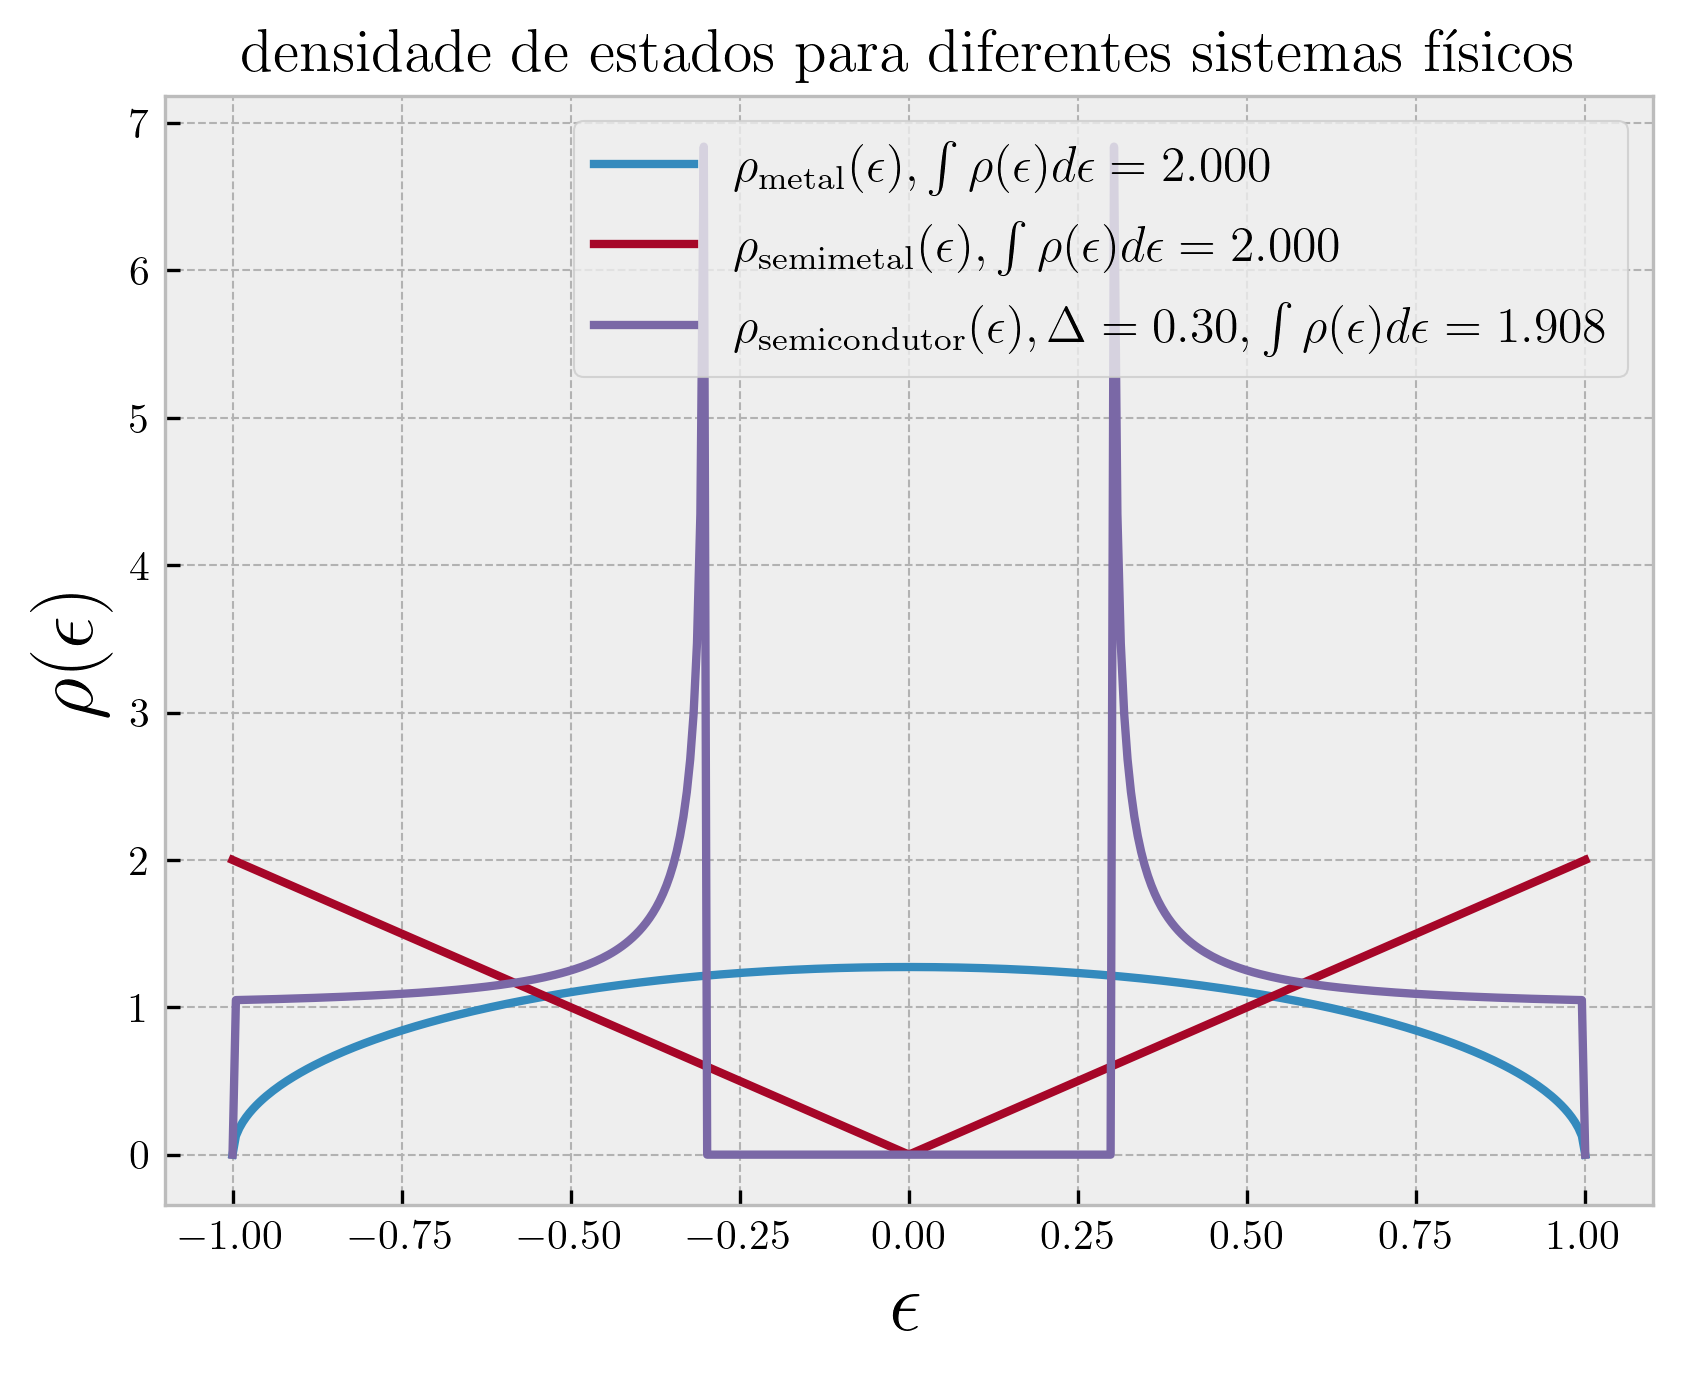
\includegraphics[width=0.6\textwidth]{fig/dos-systems.png}
\caption{Densidade de estados para os sistemas metal, semimetal e semicondutor.}
\label{fig:dos-systems}
\end{figure}
Note que obtivemos $1.999$ ao invés de $2$ para o caso semicondutor. Para fazer esse cálculo, utilizei a função \texttt{scipy.integrate.quad} e explicitei que os pontos $\pm\Delta$ são pontos de divergência. Mesmo assim a integral não resultou em $2$ exatamente.

Percebi que na verdade temos $\int \frac{x}{\sqrt{x^2-\Delta^2}} \dd{x} = \sqrt{x^2 - \Delta^2}$, de maneira que
$$
\int_{-1}^{-\Delta} \frac{\abs{\eps}}{\eps^2-\Delta^2} \dd{\eps} + \int_{\Delta}^{1} \frac{\eps}{\eps^2-\Delta^2} \dd{\eps} = 2 \sqrt{1-\Delta^2}.
$$
Assim, a integral não é exatamente $2$, a não ser que $\Delta = 0$.

\begin{figure}[H]
\centering
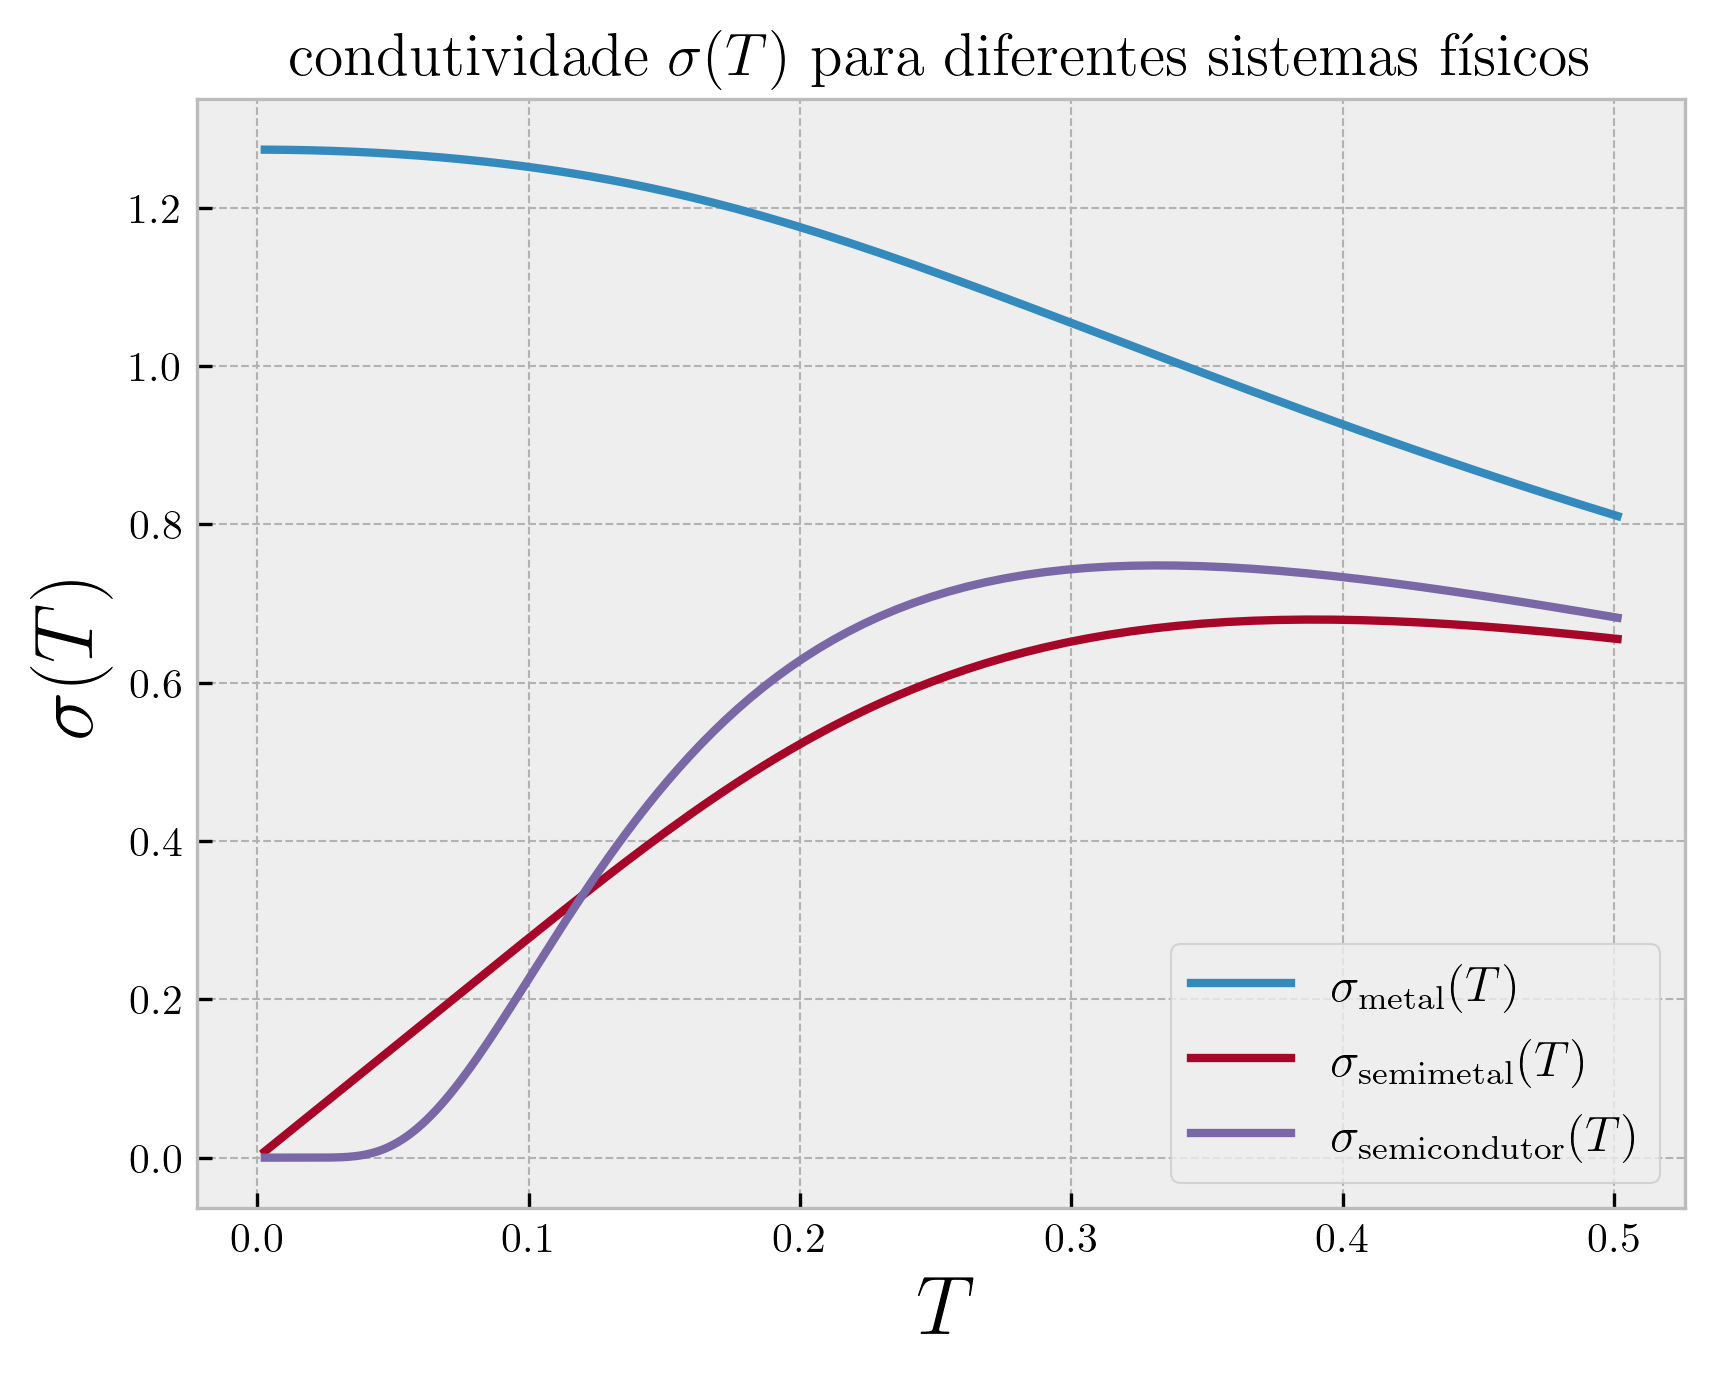
\includegraphics[width=0.75\textwidth]{fig/sigma.png}
\caption{Condutividade}
\label{fig:sigma}
\end{figure}

\end{itemize}


\pagebreak

\section{Desordem e localização de Anderson}

É intuitivo pensar que a banda associada aos operadores $d_i$ é localizada pois, na hamiltoniana considerada, existem termos de hopping entre $c_i$ e $c_j$ (sítios diferentes) e entre $c_i$ e $d_i$ (mesmo sítio), mas não existe hopping entre $d_i$ e $d_j$.

Assumindo que o espaçamento de rede é $a$, tomamos as transformadas de Fourier
$$
c_j^\d = \frac{1}{\sqrt{N}} \sum_{k} c_k^\d e^{-ikaj} \e
d_j^\d = \frac{1}{\sqrt{N}} \sum_{k} d_k^\d e^{-ikaj}.
$$

Temos então
$$
H = -t \sum_{j} \qty(c_j^\d c_{j+1} + c_{j+1}^\d c_j) +
\lambda \sum_{j} d_j^\d d_j +
V \sum_{j} \qty(c_j^\d d_j + d_j^\d c_j) \implies
$$
$$
H = \frac{1}{N} \sum_{k,k'}
\cancelto{\boxed{= N \delta_{k,k'}}}{\boxed{\sum_{j} e^{-i(k-k')ja}}}
\qty{
-t \qty(e^{ik'a} c_k^\d c_{k'} + \hc) +
\lambda \qty(d_k^\d d_{k'}) +
V \qty(c_k^\d d_{k'} + \hc)
} \implies
$$
$$
H = \sum_{k}
\qty{
-2t \cos(ka) (c_k^\d c_k) +
\lambda (d_k^\d d_k) +
V (c_k^\d d_k + d_k^\d c_k)
} \implies
$$
$$
\boxed{ H = \sum_{k}
\begin{pmatrix}
c_k^\d & d_k^\d
\end{pmatrix}
\begin{pmatrix}
-2t \cos(ka) & V \\
V & \lambda
\end{pmatrix}
\begin{pmatrix}
c_k \\ d_k
\end{pmatrix}. }
$$

Os autovalores da matriz acima são
$$
E_\pm(k) =
\frac{\qty[\lambda - 2t \cos(ka)] \pm
\sqrt{\qty[\lambda - 2t \cos(ka)]^2 + 4 V^2}}
{2}.
$$

Os mínimos e máximos de $E_{\pm}(k)$ e máximos sempre ocorrem em $k = 0$ ou $k = \pm \frac{\pi}{a}$. Assim, as larguras $d_\pm$ das respectivas bandas $\pm$ são
$$
d_\pm = \abs{E_\pm\qty(\frac{\pi}{a}) - E_\pm(0)} =
2\abs{t} \cdot \abs{1 \pm
\frac{2 \lambda}{\sqrt{(\lambda+2t)^2+4V^2}+\sqrt{(\lambda-2t)^2+4V^2}}}.
$$

Das expressões de $d_\pm$ acima, concluimos que ambas as bandas são dispersivas (possuem larguras não-nulas), a não ser que $t = 0$ ou que $\lambda \gg 1$ (nesse caso uma das bandas tem largura muito pequena e a outra uma largura da ordem de $t$).

\n

O parâmetro $V$ é o gap entre as duas bandas. Temos um isolante (em $T = 0$) quando $V \neq 0$.

O parâmetro $t$ controla a largura e o tipo das duas bandas. Quando $t > 0$ temos bandas do tipo elétron e quando $t < 0$ temos bandas do tipo buraco.

O parâmetro $\lambda$ controla o peso (assimetria) entre as duas bandas. Se $\lambda > 0$ a banda de cima tem largura maior $d_+ > d_-$. Para $\lambda < 0$ a banda de baixo tem largura maior $d_- > d_+$.

\begin{figure}[H]
\centering
\begin{subfigure}{.46\textwidth}
  \centering
  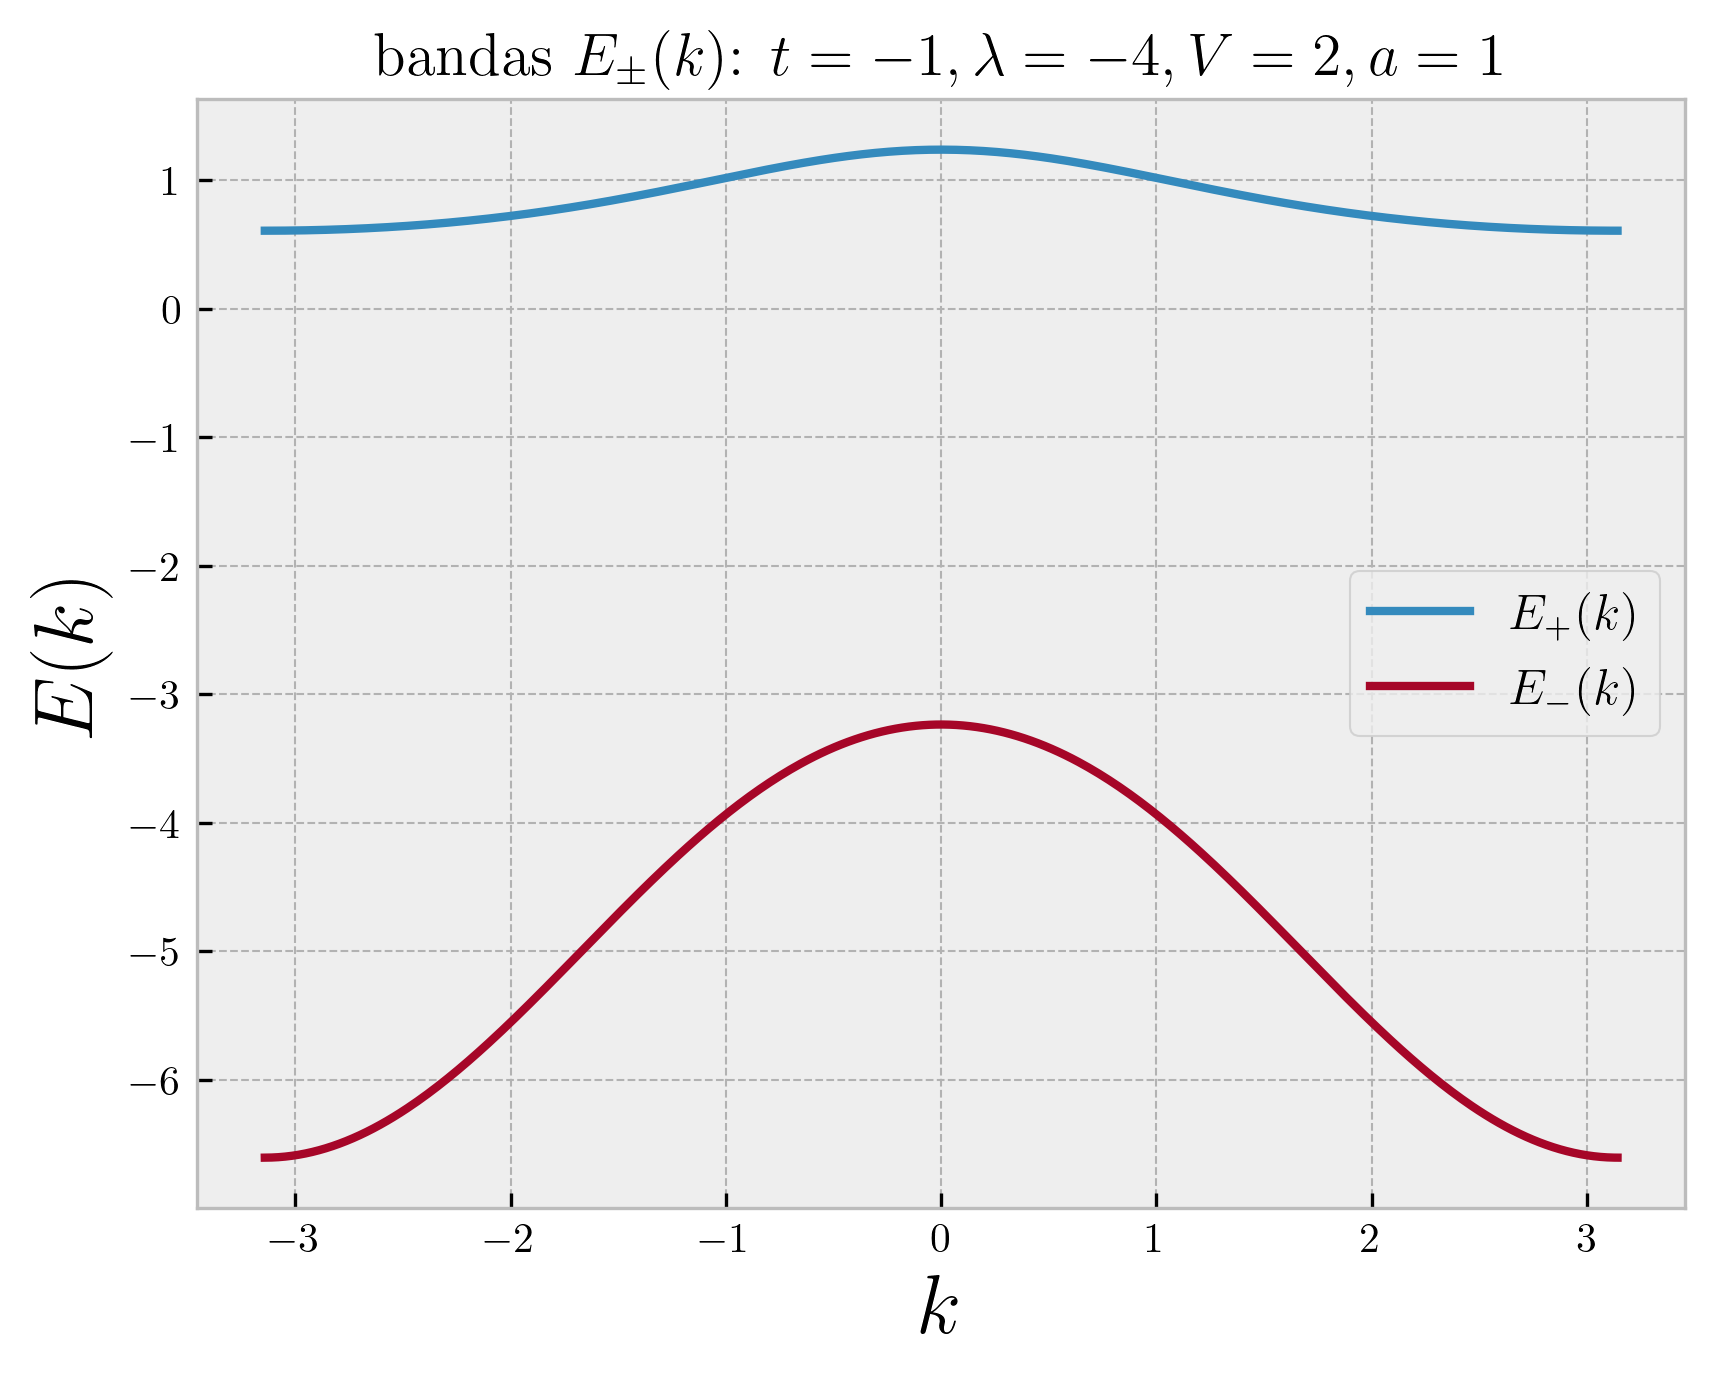
\includegraphics[width=0.95\linewidth]{fig/bandas-anderson1.png}
  \label{fig:bandas-anderson1}
\end{subfigure}
\begin{subfigure}{.46\textwidth}
  \centering
  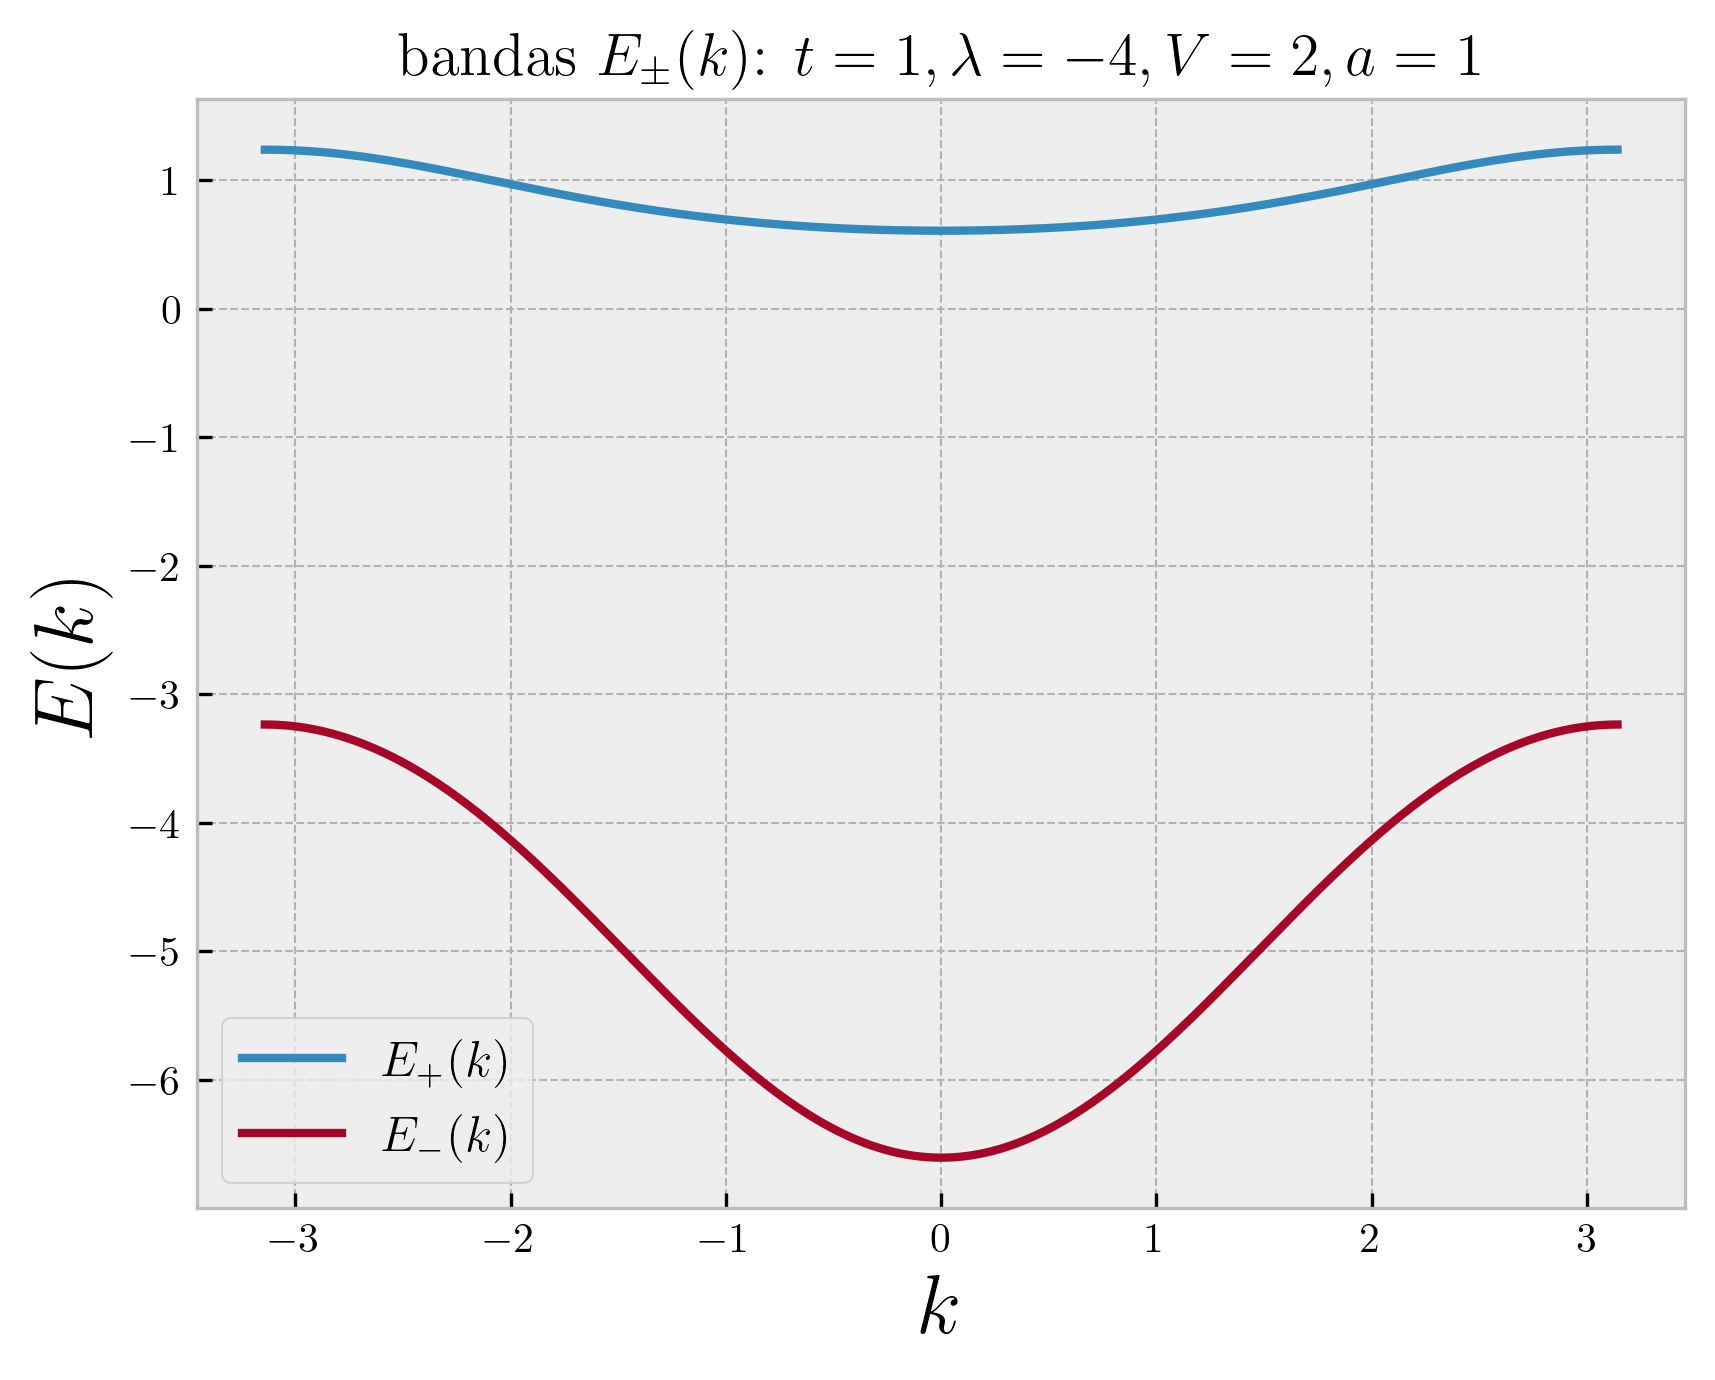
\includegraphics[width=0.95\linewidth]{fig/bandas-anderson2.png}
  \label{fig:bandas-anderson2}
\end{subfigure}
\label{fig:bandas-anderson11}
\end{figure}

\begin{figure}[H]
\centering
\begin{subfigure}{.46\textwidth}
  \centering
  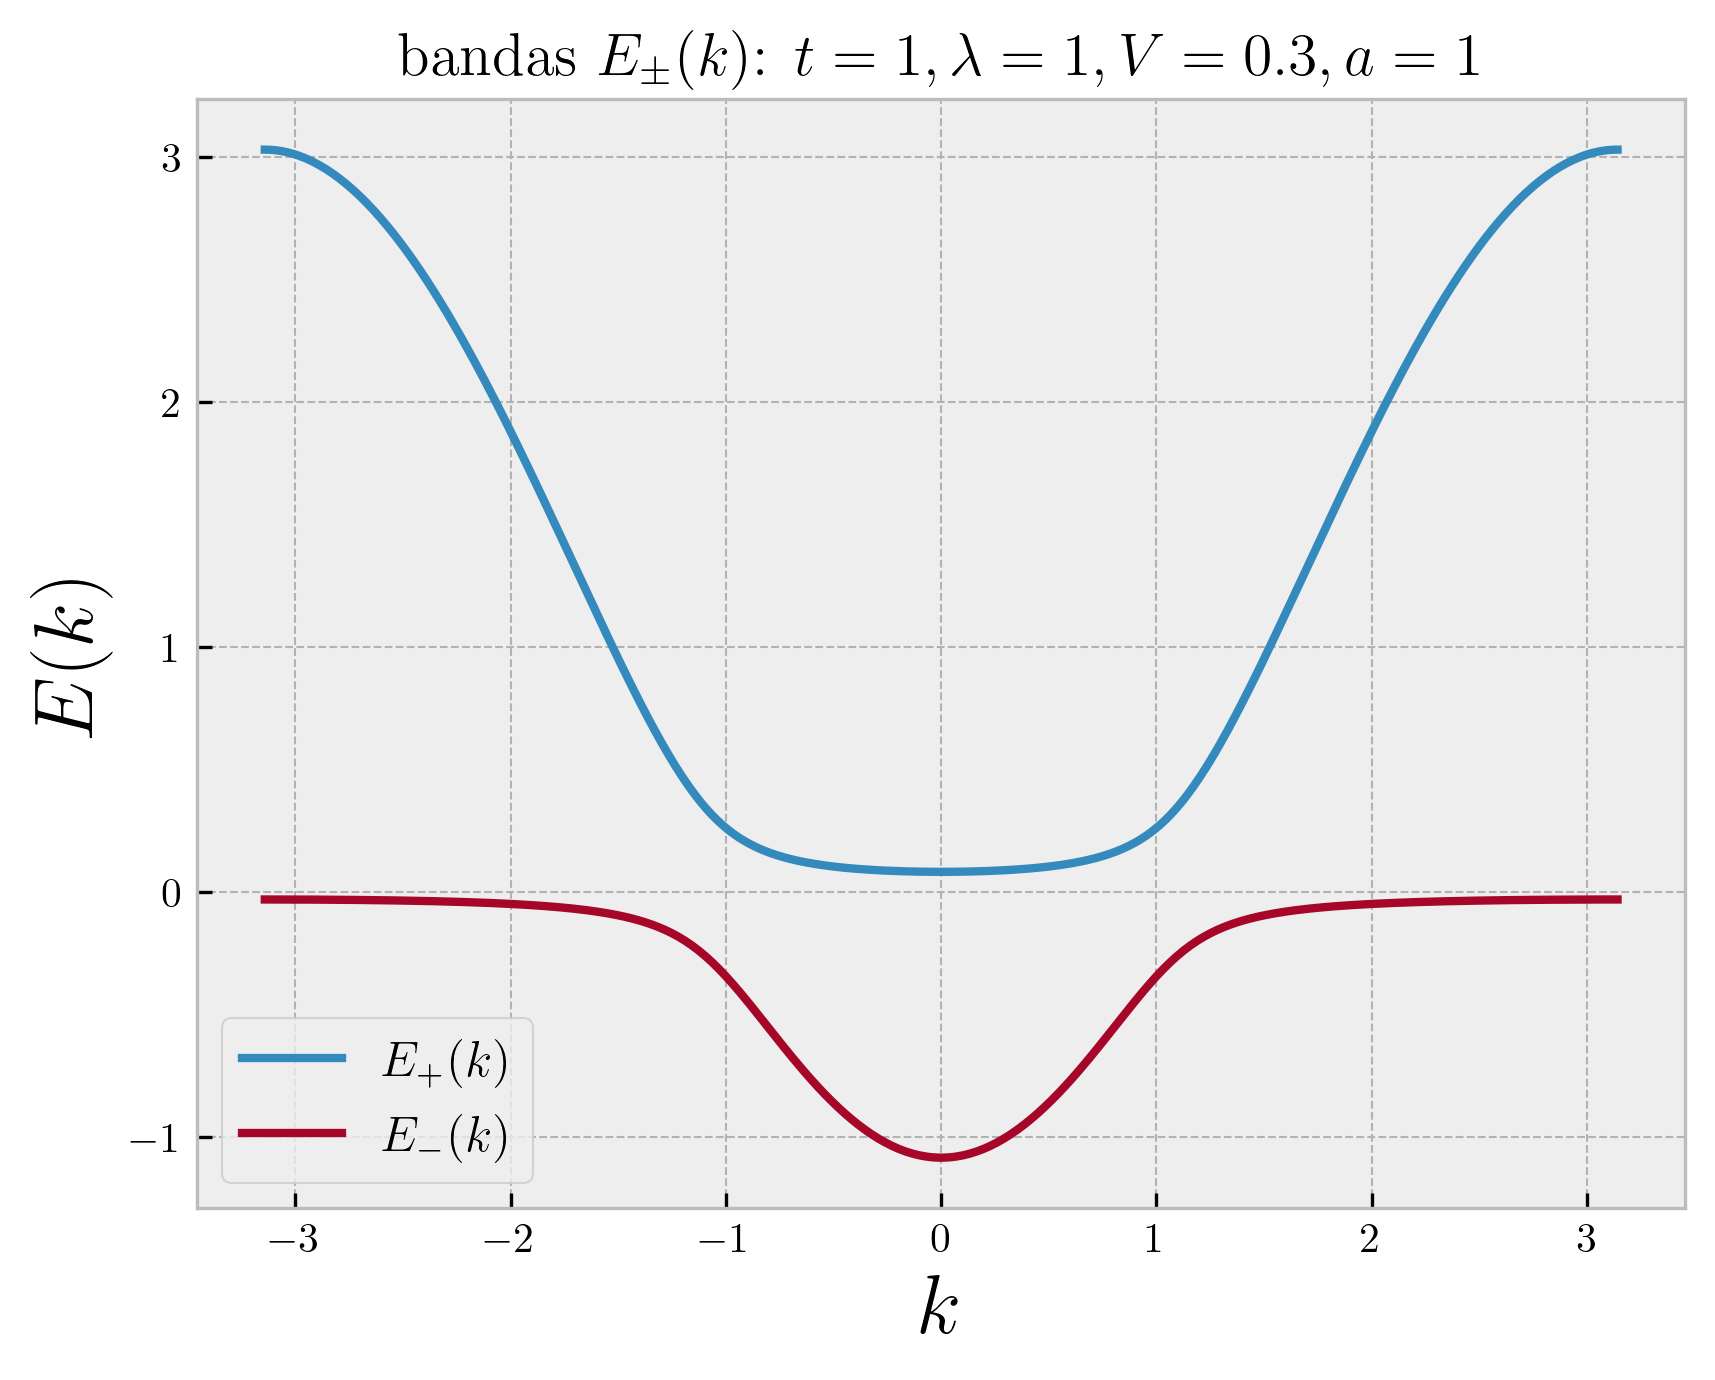
\includegraphics[width=0.95\linewidth]{fig/bandas-anderson3.png}
  \label{fig:bandas-anderson3}
\end{subfigure}
\begin{subfigure}{.46\textwidth}
  \centering
  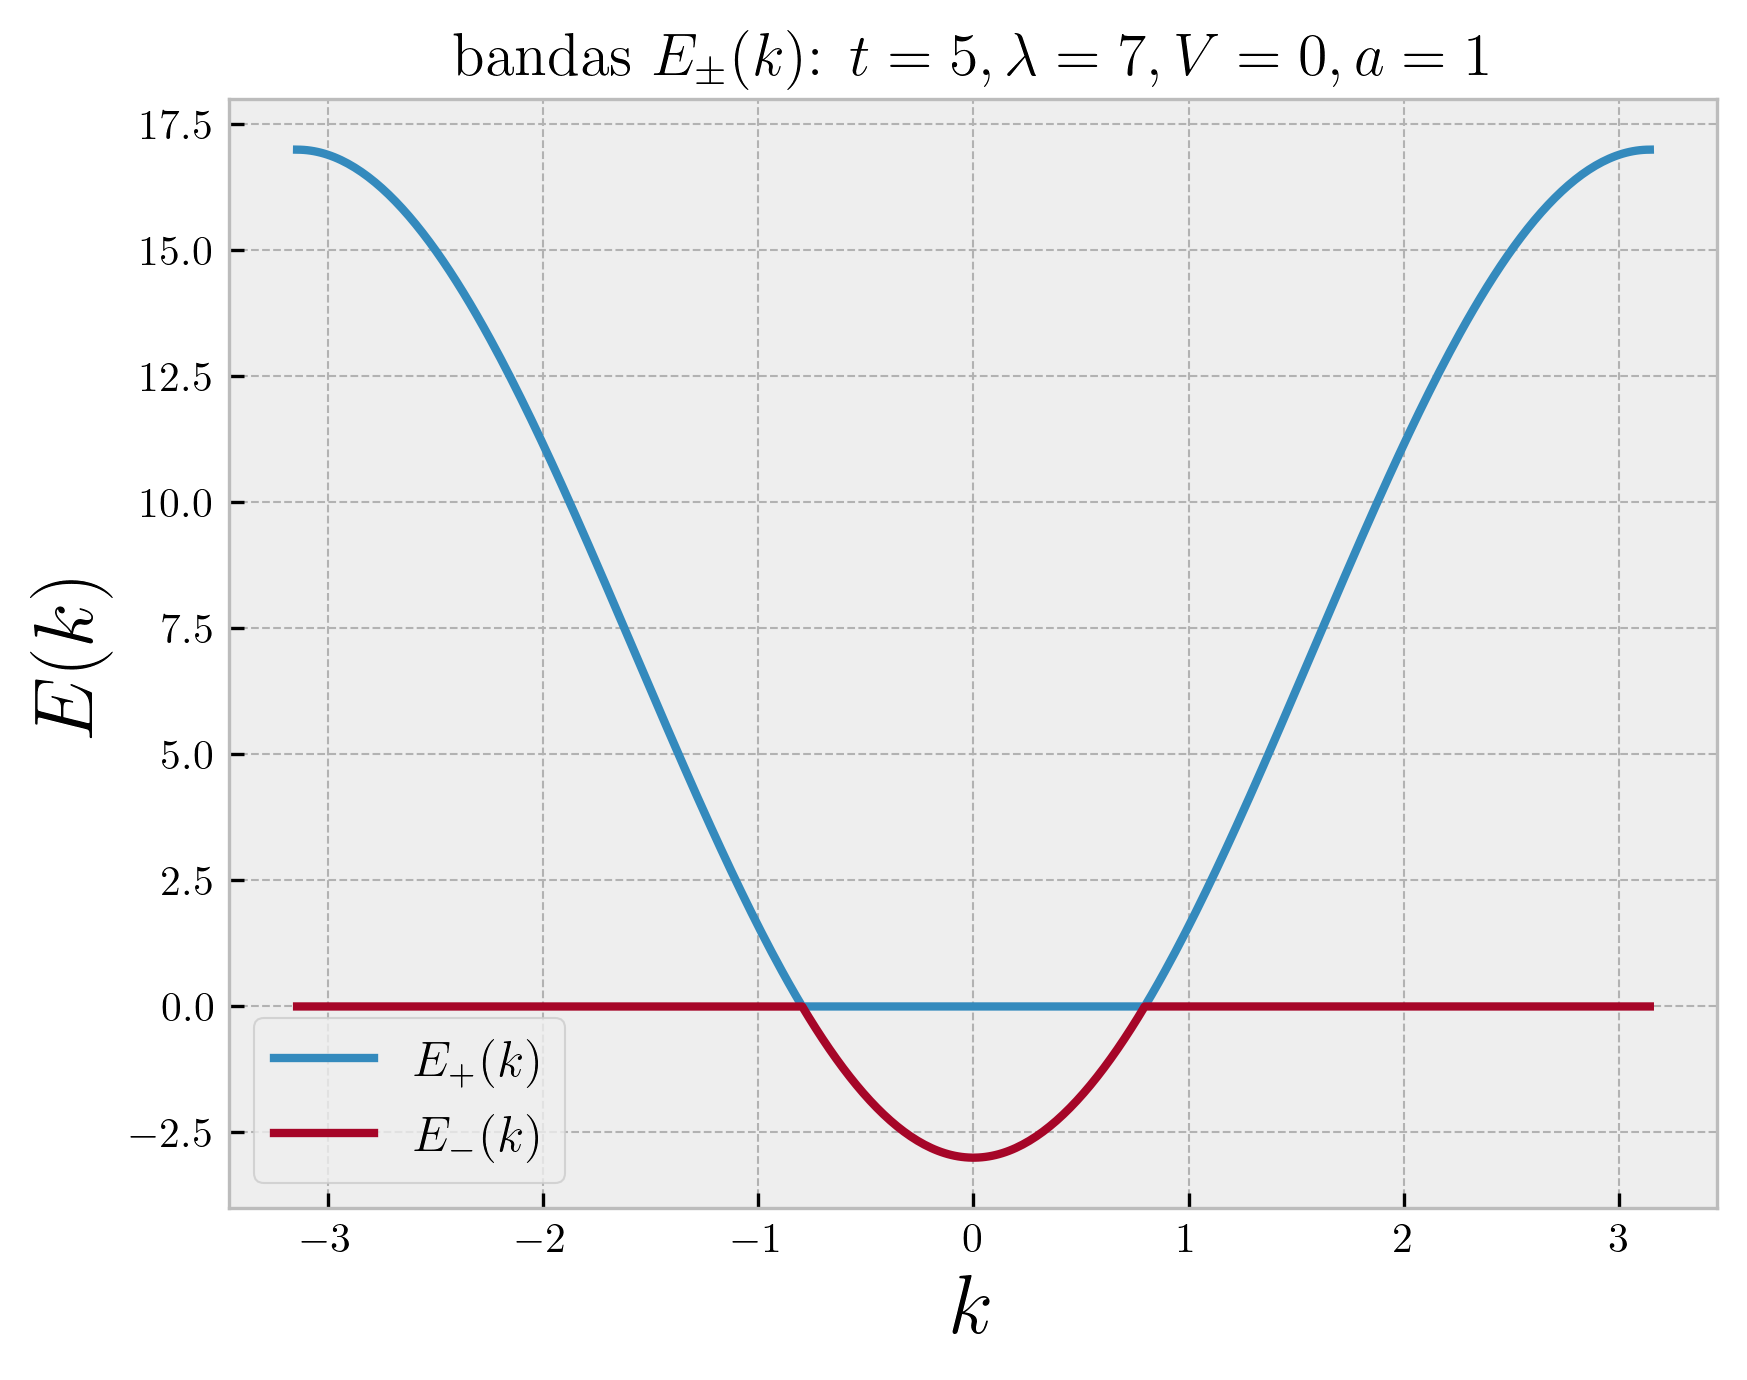
\includegraphics[width=0.95\linewidth]{fig/bandas-anderson4.png}
  \label{fig:bandas-anderson4}
\end{subfigure}
\label{fig:bandas-anderson12}
\end{figure}

(b) \textbf{FALTA O ITEM (B), TEM AQUELA FUNÇÃO $\beta(g)$}

\pagebreak

\section{Efeito Hall}

(a) A condição de quantização de Bohr-Sommerfeld nos dá que $2\pi R = n \lambda \iff k R = n$ (onde $\lambda = \frac{2\pi}{k}$ é o comprimento de onda de de Broglie). Para um elétron em 2D sob a ação de um campo magnético uniforme perpendicular ao plano, ele executará um movimento circular uniforme. Temos então que $\frac{mv^2}{R} = e v B \implies p = mv = e B R = \hbar k \implies e B R^2 = n \hbar$. O fluxo magnético é
$$
\Phi_B = B \cdot \pi R^2 = n \times \frac{h}{2e},
$$
onde $\Phi_0 = h/2e$ é o quanta de fluxo. Cada órbita com $n$ comprimento de ondas engloba $n \times \Phi_0$ de fluxo magnético.

\n

(b) Seja $c^\d$ o operador de criação em um sítio que denominamos como a origem em nosso lattice. Os operadores de criação $c_j^\d$ em outros sítios podem ser obtidos então através da aplicação do operador de translação $T(\r_j) = \exp[-\frac{i}{\hbar} \p \vdot \r_j] = \exp[-\frac{i}{\hbar} \int_{\0}^{\r_j} \p \vdot \dd{\r}]$, de maneira que
$$
c_j^\d = \exp[-\frac{i}{\hbar} \int_{\0}^{\r_j} \p \vdot \dd{\r}] c^\d.
$$
Como sabemos, podemos incluir o campo magnético através da substituição $\p \to \p - q \A$, de maneira que
$$
c_j^\d \to \exp[i\frac{q}{\hbar} \int_{\0}^{\r_j} \A \vdot \dd{\r}] c_j^\d
$$
e portanto
$$
t_{ij} c_j^\d c_i \to t_{ij} e^{i \Phi_{ij}} c_j^\d c_i, \quad
\Phi_{ij} = \frac{q}{\hbar}\int_{\r_i}^{\r_j} \A \vdot \dd{\r}.
$$

Do item (a) temos que
$$
n \Phi_0 = \Phi_B = \iint \B \vdot \dd{\vb{S}} = \iint (\curl{\A}) \vdot \dd{\vb{S}} = \oint \A \vdot \dd{\r} \implies n \propto \Phi_{jj}.
$$

O gauge de Landau é $\A = Bx \vu{y}$. O modelo tight-binding da rede quadrada em 2D para primeiros vizinhos então nos dá
$$
\Phi_{(x,y),(x+a,y)} = \frac{q}{\hbar} \int_{(x,y)}^{(x+a,y)} (B x \vu{y}) \vdot (dx \vu{x}) = 0
$$
$$
\Phi_{(x,y),(x,y+a)} = \frac{q}{\hbar} \int_{(x,y)}^{(x,y+a)} (B x \vu{y}) \vdot (dy \vu{y}) = \frac{qBxa}{\hbar}.
$$
<++>
$$
H = -t \sum_{\R}
\qty{
\qty[c^\d_{(\R+a\vu{x})} c_{\R} + c_{\R}^\d c_{(\R+a\vu{x})}] +
\qty[e^{i\frac{qBxa}{\hbar}} c^\d_{(\R+a\vu{y})} c_{\R} + e^{-i\frac{qBxa}{\hbar}}c_{\R}^\d c_{(\R+a\vu{y})}]
}
$$
$$
H = -\frac{t}{N} \sum_{\k,\k'}
\qty{
\qty[
\cancelto{\boxed{= N \delta_{\k,\k'}}}{\boxed{\sum_{\R} e^{-i(\k-\k')\vdot\r}}}
e^{-ik_x a} c_{\k}^\d c_{\k'} + \hc] +
\qty[
\cancelto{\boxed{= N \delta_{\k-\frac{qBa}{\hbar}\vu{x},\k'}}}{\boxed{\sum_{\R} e^{-i\qty(\k-\k'-\frac{qBa}{\hbar}\vu{x})\vdot\r}}}
e^{-ik_y a} c_{\k}^\d c_{\k'} + \hc]
}
$$

\textbf{NÃO TENHO MUITO IDEIA da DOS. VOU INVENTAR QUALQUER COISA}

\pagebreak

\section{Número de Chern para um modelo de duas bandas}

É direto obter que
$$
\abs{\vb{h}(\vb{k})}^2 =
\Delta^2 + 2 (1 + \cos k_x \cos k_y - \Delta (\cos k_x + \cos k_y)) + \Delta^2.
$$
$$
\begin{vmatrix}
h_x & h_y & h_z \\
\pdv{h_x}{k_x} & \pdv{h_y}{k_x} & \pdv{h_z}{k_x} \\
\pdv{h_x}{k_y} & \pdv{h_y}{k_z} & \pdv{h_z}{k_y} \\
\end{vmatrix}
=
\begin{pmatrix}
\sin k_x & \sin k_y & \Delta - \cos k_x - \cos k_y \\
\cos k_x &  0 & \sin k_x \\
0 & \cos k_y & \sin k_y \\
\end{pmatrix}
=
\Delta \cos k_x \cos k_y - \cos k_x - \cos k_y.
$$

Portanto,
$$
C = \frac{1}{4\pi} \int_{-\pi}^{\pi} \int_{-\pi}^{\pi}
\frac{\Delta \cos k_x \cos k_y - \cos k_x - \cos k_y}{\qty[\Delta^2 + 2 (1 + \cos k_x \cos k_y - \Delta (\cos k_x + \cos k_y)) + \Delta^2]}
\dd{k_x} \dd{k_y}
$$

Integrando a expressão acima numericamente com a função \texttt{scipy.integrate.dblquad} do Python, obtemos a Figura \ref{fig:chern}:
\begin{figure}[H]
\centering
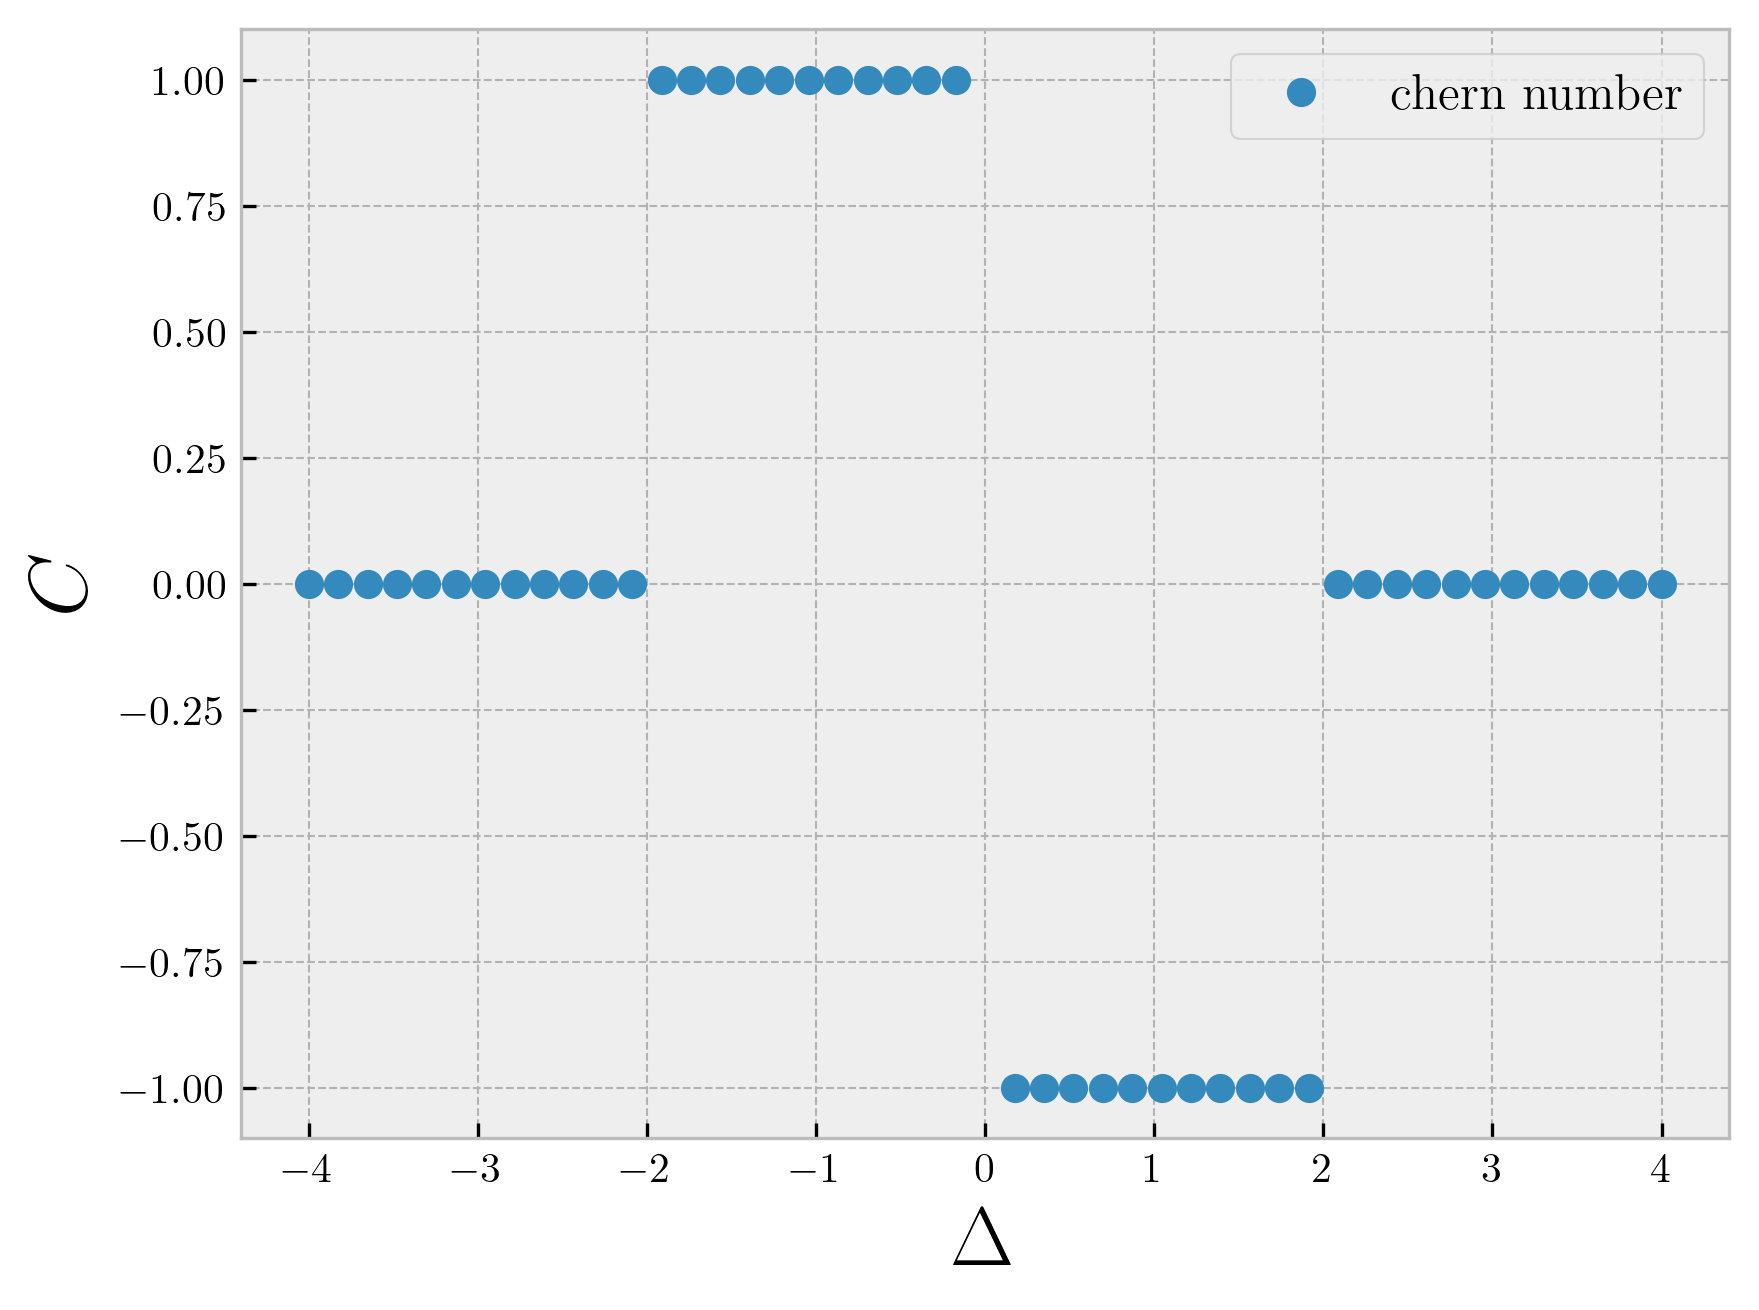
\includegraphics[width=0.75\textwidth]{fig/chern.png}
\caption{Número de Chern em função do parâmetro $\Delta$.}
\label{fig:chern}
\end{figure}

\pagebreak

\section{Condutividade Hall}

Da equação \ref{eq:cond}, substituindo $\grad_{\k}f = \pdv{f(\k)}{\eps_n(\k)} \grad_{\k}\eps_n(\k)$ ($f$ é a distribuição de Fermi-Dirac), $\v_n(\k) = \frac{1}{\hbar} \grad_{\k}\eps_n(\k)$ e aproximando $1-i\omega\tau \approx -i\omega\tau$ no limite $\omega\tau \gg 1$, temos
$$
\bm{\s}^{(n)}(\omega) = \frac{e^2}{i\omega \hbar^2}
\int \frac{\dd[2]{\k}}{(2\pi)^2} \grad_{\k}\eps_n(\k) \grad_{\k} f.
$$

 Integrando por partes as componentes $\mu, \nu$:
$$
\int \dd[2]{\k} \pdv{\eps_n(\k)}{k_\mu} \pdv{f(\k)}{k_\nu} =
\cancelto{0}{\boxed{\int \dd[2]{\k} \pdv{k_\nu} \qty[\pdv{\eps_n(\k)}{k_\mu} f(\k)]}} -
\int \dd[2]{\k} \pdv{\eps_n(\k)}{k_\mu}{k_\nu} f(\k).
$$

O termo superficial acima é zero pois o integrando é periódico dentro na borda da zona de Brillouin.

Em $T=0$, a distribuição de Fermi-Dirac faz a integral ser somente sobre os estados ocupados, portanto
$$
\s^{(n)}_{\mu\nu}(\omega) = \frac{e^2}{i\omega \hbar^2}
\int \frac{\dd[2]{\k}}{(2\pi)^2} \pdv{\eps_n(\k)}{k_\mu} \pdv{f(\k)}{k_\nu} =
- \frac{e^2}{i\omega}
\int_{\text{ocupados}} \frac{\dd[2]{\k}}{(2\pi)^2} \frac{1}{\hbar^2} \pdv{\eps_n(\k)}{k_\mu k_\nu}.
$$

O resultado do problema 3(b) da Lista 3 para o tensor massa efetiva é
$$
\frac{1}{\hbar^2} \pdv{\eps_n(\k)}{k_\mu}{k_\nu} =
\frac{\delta_{\mu\nu}}{m_e} +
\qty(\frac{\hbar}{m_e})^2
\sum_{m\neq n}
\frac{
\mel**{n}{\frac{1}{i}\pdv{r_\mu}}{m} \mel**{m}{\frac{1}{i}\pdv{r_\nu}}{n} +
\mel**{n}{\frac{1}{i}\pdv{r_\nu}}{m} \mel**{m}{\frac{1}{i}\pdv{r_\mu}}{n}
}{\eps_n(\k) - \eps_{m}(\k)}.
$$

O problema que estamos tratando envolve um campo elétrico alternado $\E(t) = \E(\omega) e^{-i\omega t}$, ou seja, uma frequência $\omega$ de onda eletromagnética bem definida. A essa frequência correspondem excitações de energia $\delta(\pm \hbar \omega + \eps_n(\k) - \eps_m(\k))$ do espectro. No limite $\hbar \omega \to 0$, então é razoável aproximarmos
$$
\frac{1}{\hbar^2} \pdv{\eps_n(\k)}{k_\mu}{k_\nu} =
\frac{\delta_{\mu\nu}}{m_e} +
\qty(\frac{\hbar}{m_e})^2
\sum_{m\neq n} \qty{
\frac{\mel**{n}{\frac{1}{i}\pdv{r_\mu}}{m} \mel**{m}{\frac{1}{i}\pdv{r_\nu}}{n}}
{\hbar \omega + \eps_n(\k) - \eps_{m}(\k)} +
\frac{\mel**{n}{\frac{1}{i}\pdv{r_\nu}}{m} \mel**{m}{\frac{1}{i}\pdv{r_\mu}}{n}}
{-\hbar \omega + \eps_n(\k) - \eps_{m}(\k)}
} .
$$

Expandimos então para $\hbar \omega \to 0$:
$$
\frac{1}{\pm \hbar \omega + \eps_n(\k) - \eps_m(\k)} =
\boxed{\frac{1}{\eps_n(\k) - \eps_m(\k)}}
\mp \frac{\hbar\omega}{(\eps_n(\k) - \eps_m(\k))^2}.
$$

Como estamos interessados na condutividade $\s_{xy}$, note que ela deve se manter a invariante sobre a rotação $x \to y$, $y \to -x$. Mas, com relação ao primeiro termo destacado acima, as derivadas $\pdv{x}$ e $\pdv{y}$ tomam um sinal de menos na expressão de $\s_{y,-x}$, de maneira que o termo destacado é anulado.

Além disso, da equação de Heisenberg temos $i\hbar \dot{r}_\mu = [r_\mu, H] = i\hbar \pdv{H}{p_\mu} \implies \dot{r}_\mu = \pdv{H}{p_\mu}$. Podemos então fazer a substiuição $p_\mu = \frac{1}{i} \hbar \pdv{r_\mu} = m_e \dot{r}_\mu = m_e \pdv{H}{p_\mu} = m_e \hbar^{-1} \pdv{H}{k_\mu}$.

Dessa maneira, ficamos com
$$
\s^{(n)}_{xy}(T=0) =i\frac{e^2}{\hbar}\int_{\text{BZ}}\frac{\dd[2]{\k}}{(2\pi)^2}
\sum_{m\neq n}
\qty[
\frac{
\mel**{n}{\partial_x H}{m} \mel**{m}{\partial_y H}{n} -
\mel**{n}{\partial_y H}{m} \mel**{m}{\partial_x H}{n}
}{(\eps_n(\k) - \eps_{m}(\k))^2} ]
$$

Usando que $(E_n - E_m)^2 = 4h^2$ e a equação (26) das notas de aula sobre Isolantes Topológicos para a curvatura de Berry, chegamos que
$$
\s^{(n)}_{xy}(T=0) =
\frac{e^2}{\hbar} \int_{\text{BZ}} \frac{\dd[2]{\k}}{(2\pi)^2} B_n(\k) =
\frac{e^2}{\hbar} C_n.
$$

\textbf{DAR UMA LIMPADA NO TEXTO.}



\end{document}
